\documentclass[tikz,border=2pt]{standalone}
\usepackage{amsmath}
\usetikzlibrary{arrows.meta}
\begin{document}
% Anatomy of the Prisoner's Dilemma bimatrix: rows S_1 (player 1, blue), columns S_2 (player 2, red),
% cell (s_1,s_2) holds v_1(s_1,s_2), v_2(s_1,s_2). Player 1 compares first entries down a column
% (here -2 vs -1 in column M), player 2 compares second entries along a row (-5 vs -4 in row F).
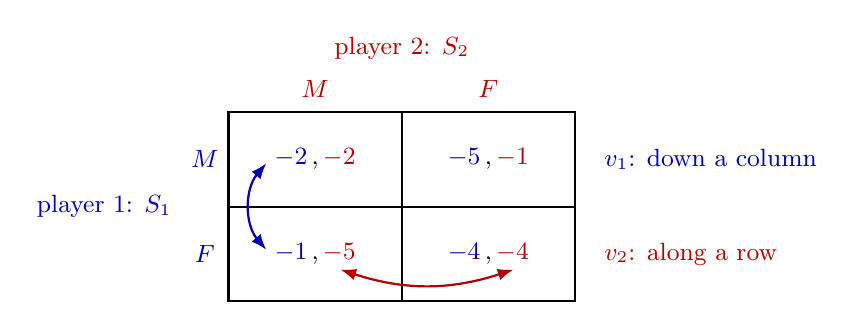
\begin{tikzpicture}[font=\small, >={Latex[length=2mm]}]
  \def\w{2.2} \def\h{1.2}
  \draw[thick] (0,-\h) rectangle (2*\w,\h);
  \draw[thick] (\w,-\h) -- (\w,\h);
  \draw[thick] (0,0) -- (2*\w,0);
  % strategy labels
  \node[red!70!black] at (0.5*\w,\h+0.3) {$M$};
  \node[red!70!black] at (1.5*\w,\h+0.3) {$F$};
  \node[blue!70!black] at (-0.3,0.5*\h) {$M$};
  \node[blue!70!black] at (-0.3,-0.5*\h) {$F$};
  \node[red!70!black, anchor=south] at (\w,\h+0.55) {player 2: $S_2$};
  \node[blue!70!black, anchor=east] at (-0.6,0) {player 1: $S_1$};
  % payoffs v_1, v_2
  \foreach \x/\y/\a/\b in {0.5/0.5/-2/-2, 1.5/0.5/-5/-1, 0.5/-0.5/-1/-5, 1.5/-0.5/-4/-4}
    \node at (\x*\w,\y*\h) {\textcolor{blue!70!black}{$\a$}\,,\,\textcolor{red!70!black}{$\b$}};
  % player 1 compares first entries down column M
  \draw[<->, blue!70!black, thick] (0.5*\w-0.62,0.5*\h-0.05) to[bend right=40] (0.5*\w-0.62,-0.5*\h+0.05);
  % player 2 compares second entries along row F
  \draw[<->, red!70!black, thick] (0.5*\w+0.32,-0.5*\h-0.2) to[bend right=18] (1.5*\w+0.32,-0.5*\h-0.2);
  % reading rules
  \node[blue!70!black, anchor=west] at (2*\w+0.25,0.5*\h) {$v_1$: down a column};
  \node[red!70!black, anchor=west] at (2*\w+0.25,-0.5*\h) {$v_2$: along a row};
\end{tikzpicture}
\end{document}
